\documentclass[a4paper,12pt]{article}
\usepackage[a4paper,margin=3cm]{geometry}
\usepackage[square, sort&compress, numbers]{natbib}
%\documentclass[a4paper]{bio}
% \usepackage[colorlinks=true, urlcolor=citecolor, linkcolor=citecolor, citecolor=citecolor]{hyperref}
\usepackage{url}
\usepackage{rotating}
\usepackage{array}
\usepackage{setspace} 
\usepackage{lineno}
\usepackage{rotating}
\usepackage{multirow}
\usepackage{color}
\usepackage{colortbl}
\usepackage{amssymb}
\usepackage{xcolor}


\linenumbers

\setlength\parindent{0ex}
\setlength\parskip{2ex}
\renewcommand{\baselinestretch}{1}

\newcolumntype{L}[1]{>{\raggedright\let\newline\\\arraybackslash\hspace{0pt}}m{#1}}
\newcolumntype{C}[1]{>{\centering\let\newline\\\arraybackslash\hspace{0pt}}m{#1}}
\newcolumntype{R}[1]{>{\raggedleft\let\newline\\\arraybackslash\hspace{0pt}}m{#1}}



\newcommand{\inputtable}[1]{\input{#1} }

%\def\figdiscrim{\ref{fig:discrim}}
%\def\figIalone{\ref{figIalone}}
%\def\tabIinteractions{\ref{tabIinteractions}}
%\def\tabHalone{\ref{tabHalone}}
%\def\tabHinteractions{\ref{tabHinteractions}}
%\def\tabOalone{\ref{tabOalone}}
%\def\tabUalone{\ref{tabUalone}}

\def\jid{0}
\newcommand{\inputtable}[1]{}

\def\figdiscrim{1}
\def\figIalone{2}
\def\tabIinteractions{1}
\def\tabHalone{2}
\def\tabHinteractions{3}
\def\tabOalone{4}
\def\tabUalone{5}


\def\nocase{no case}
\newcommand{\new}[1]{\textcolor{red}{#1}}  

\begin{document}
\doublespacing
% Title of paper: 160 CHARACTERS AND SPACES
%Real-life protection provided by vaccination, booster doses and previous infection against covid-19 infection, hospitalisation or death over time in the Czech Republic: a whole country retrospective view \\[2ex]

{\noindent \Large\bf Protection by vaccines and previous infection against the Omicron variant of SARS-CoV-2 \\[2ex]
{\normalsize Article type: Major article}\\[1ex]
{\normalsize Running head: Protection against Omicron}\\[1ex]
{\normalsize Word count of the abstract: 200} \\[1ex]
{\normalsize Word count of the text: 3353}}\\[2ex]
{\large Martin \v{S}m\'id$^{1,2,*}$, Lud\v{e}k Berec$^{2,3,4}$,  Lenka P\v{r}ibylov\'a$^5$, Ond\v{r}ej M\'ajek$^{6,7}$, Tom\'a\v{s} Pavl\'{\i}k$^{6,7}$, Ji\v{r}\'{\i} Jarkovsk\'y$^{6,7}$, Jakub Weiner$^{2,8}$, Tamara Barusov\'{a}$^{9,10}$, Jan Trnka$^{11}$} \\[2ex]
$^1$Czech Academy of Sciences, Institute of Information Theory and Automation, Pod Vodárenskou věží 4, 18200 Praha 8, Czech Republic \\[1ex]
$^2$Centre for Modelling of Biological and Social Processes, Na břehu 497/15, 19000 Praha 9, Czech Republic \\[1ex] 
$^3$Centre for Mathematical Biology, Institute of Mathematics, Faculty of Science,  University of South Bohemia, Branišovská 1760, 37005 České Budějovice, Czech Republic \\[1ex]
$^4$Czech Academy of Sciences, Biology Centre, Institute of Entomology, Department of Ecology, Branišovská 31, 37005 České Budějovice, Czech Republic \\[1ex]
$^5$Department of Mathematics and Statistics, Faculty of Science, Masaryk University, 61137 Kotl\'a\v{r}sk\'a 2, Brno, Czech Republic \\[1ex]
$^6$Institute of Biostatistics and Analyses, Faculty of Medicine, Masaryk University, Kamenice 126/3, 62500 Brno, Czech Republic \\[1ex]
$^7$Institute of Health Information and Statistics of the Czech Republic, Palackého náměstí 4, 12801 Praha 2, Czech Republic \\[1ex] 
$^8$Siesta Labs, Konopišťská 739/16, 10000 Praha 10, Czech Republic \\[1ex] 
$^9$First Faculty of Medicine, Charles University, Kate\v{r}inská 32, 12108 Praha 2, Czech Republic \\[1ex]
$^{10}$Czech Academy of Sciences, Institute of Computer Science, Department of Statistical Modelling, Pod Vodárenskou věží 2, 18207 Praha 8, Czech Republic \\[1ex]
$^{11}$Department of Biochemistry, Cell and Molecular Biology, Third Faculty \\ of Medicine, Charles University, Ruská 87, 10000 Praha 10, Czech Republic \\[3ex]
%\newpage
%\begin{abstract}
\noindent
%\hrule 
\vspace{1ex}
\noindent
{\bf ABSTRACT} \\[1ex]
{\bf Background.} The Omicron variant of SARS-CoV-2 evades immunity conferred by vaccines and previous infections. \\
{\bf Methods.} We used a Cox proportional hazards model and a logistic regression on individual-level population-wide data from the Czech Republic to estimate risks of infection and hospitalization, including severe states.\\
{\bf Results.} A recent ($<2$ months) full vaccination reached VE 43\% (95\% CI: 42-44) against infection by Omicron compared to 73\% (CI: 72-74) against Delta. A recent booster increased VE to 56\% (CI: 55-56) against Omicron infection compared to 90\% (CI: 90-91) for Delta. The VE against Omicron hospitalization of a recent full vaccination was 45\% (95\% CI: 29-57), with a recent booster 87\% (CI: 84-88). The VE against the need for oxygen therapy due to Omicron was 57\% (CI: 32-72) for recent vaccination, 90\% (CI: 87-92) for a recent booster. Post-infection protection against Omicron hospitalization declined from 68\% (CI: 68-69) at $<6$ months to 13\% (CI: 11-14) at $>6$ months after a previous infection. The OR for Omicron relative to Delta was 0.36 (CI: 0.34-0.38) for hospitalization, 0.24 (CI: 0.22-0.26) for oxygen, and 0.24 (CI: 0.21-0.28) for ICU admission.\\
{\bf Discussion.} Recent vaccination still brings substantial protection against severe outcome for Omicron.
\\[1ex]
{\bf Keywords.} covid-19; post-infection immunity; vaccine effectiveness; SARS-CoV-2; Omicron variant; hospitalization. \\[1ex]
%{\bf Funding} {\rm No external funding was used to conduct this study.} 
%\hrule
%\vspace{1ex}
%\end{abstract}

% \newpage 
\setlength{\parindent}{0cm}

\section*{INTRODUCTION}
\label{sec1}

\doublespacing


The B.1.1.529 (Omicron) variant of SARS-CoV-2 was first detected in South Africa in November 2021, immediately designated a variant of concern by the WHO \citep{who2021omicron} and  thereafter seen quickly to spread throughout most of the world. This rapid spread was at least in part brought about by a degree of immune evasion due to a large number of mutations in the viral S-protein, which led to changes in epitopes recognised by antibodies elicited by vaccination or previous infection \citep{mccallum2022}. Together with non-pharmacological interventions such as face masks, distancing, ventilation of interior spaces testing and isolating, vaccination is among the most effective means of individual and collective protection from the impacts of the pandemic. The immune evasion by the Omicron variant thus caused concern and led to a lot of interest in both laboratory and real-life epidemiological data that could accurately measure this phenomenon.
\label{sec1}

Since December 27, 2020 the inhabitants of the Czech Republic have been receiving covid-19 vaccines with the largest number vaccinated with the mRNA vaccine BNT162b2 (Pfizer/BioNTech), followed by mRNA-1273 (Moderna), and the adenovirus-based vector vaccines ChAdOx1 nCoV-19 (AstraZeneca) and Ad26.CoV2.S (Johnson\&Johnson) \citep{mzcr}. By February 13, 2022, the end of our study period, 68\% of the population had a complete vaccination and 39\% received a booster dose  \citep{mzcr} 

The first case of the Omicron variant in the Czech Republic was detected at the end of November 2021, its proportion of recorded cases rapidly rose and by January 10, 2022 it became the dominant variant  (Fig. \figdiscrim). An increasing number of infections among fully vaccinated and re-infections indeed suggests that immune evasion poses a significant risk to further covid-19 development \citep{mzcr}. 

In this study, we estimate how the protection due to vaccination or previous SARS-CoV-2 infection against covid-19 infection, hospital admission, oxygen therapy and ICU admission varies in relation to the virus variant and time elapsed for the whole population of the Czech Republic.
\ifthenelse{\jid=1}{}{
\begin{figure*}
\centering
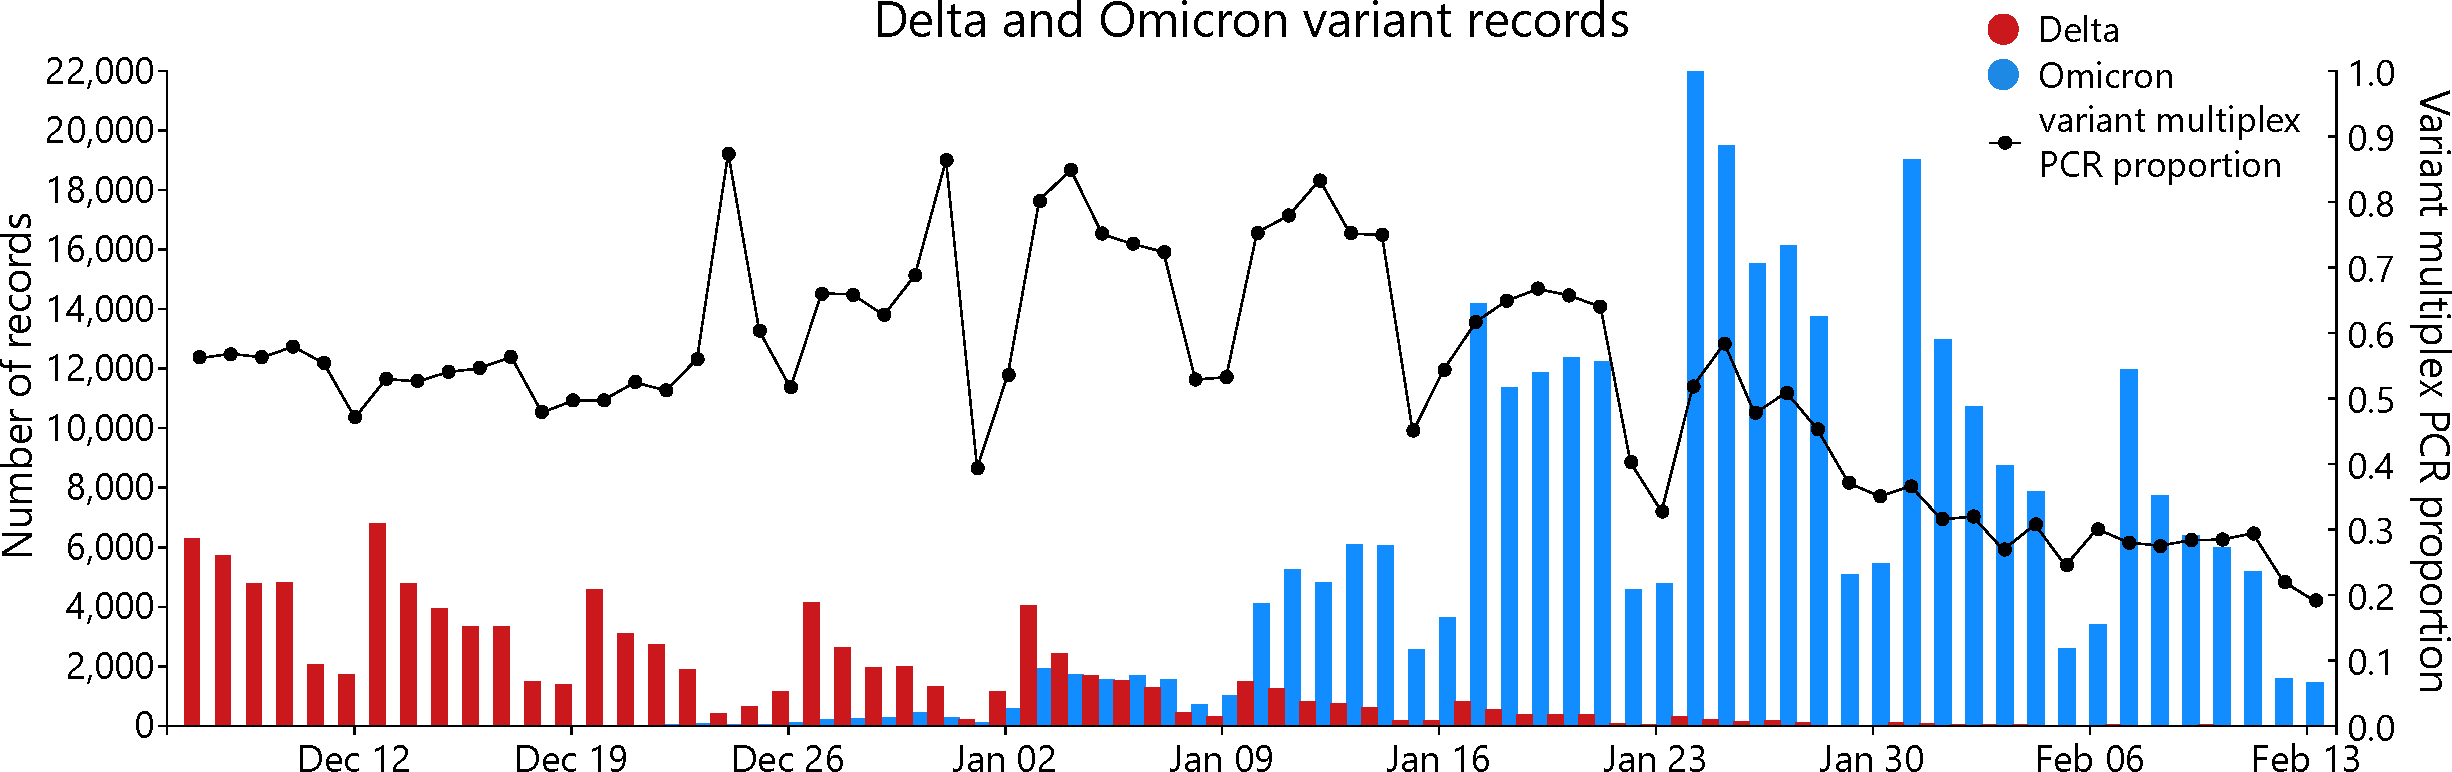
\includegraphics[width=0.85\textwidth]{smid_protection_against_omicron_fig1.pdf}
\caption{Number of recorded cases with assigned Delta (red) and Omicron (blue) variant and the proportion of PCR positive tests (black) tested for viral variants using multiplex PCR.}
\label{fig:discrim}
\end{figure*}}


\section*{METHODS}
\label{sec2}

\subsection*{Study population and data sources}

The analyses are based on data from the Czech National Information System of Infectious Diseases (ISID), which includes records of all individuals tested positive for SARS-CoV-2 in the Czech Republic since the beginning of covid-19 pandemic, including children \citep{komenda2020}. This database is overseen by the Czech Ministry of Health and operated by the Institute of Health Information and Statistics of the Czech Republic. Data are routinely collected in compliance with Czech legal regulations (Act on the Protection of Public Health). The Director of the Institute of Health Information and Statistics of the Czech Republic has granted that there non need of an ethical approval of the retrospective analyses presented in this paper.

The ISID database collects demographic data (age, sex and region of residence), dates of vaccination, including the vaccine types for each dose, and dates of infection and potential reinfection, hospitalization including treatment type and the date of potential death with covid-19. The data recorded in the study period include information on whether the infection is caused by the Omicron, Delta, some other variant, or that a variant discrimination was not performed, see Figure \figdiscrim. The information on the variant is based on results of multiplex PCR or viral genome sequencing, which are available only for a subset of all PCR-positive cases. The variants were identified using the definition of viral S-protein mutations according to ECDC \citep{ECDC_var_concern}; the algorithm was tailored to multiplex PCR kits used in the Czech Republic in collaboration with the National Institute of Public Health and the National Reference Laboratory \citep{SZU_zprava}. Additional information on deaths from any cause come from the Death Certificate System; these data are used for censoring purposes only.

\subsection*{Study endpoints}

We studied four types of events: (i) SARS-CoV-2 infection defined as a PCR-confirmed positive test of any type of sample regardless of the presence of symptoms, (ii) hospital admission of a person, who tested positive on a PCR test, within two weeks after the confirmed infection or earlier, (iii) use of any type of oxygen therapy (nasal oxygen, noninvasive ventilation, invasive mechanical ventilation, high-flow nasal oxygen, and extracorporeal membrane oxygenation) and (iv) admission to ICU during the hospitalization. All events were related to the date of infection report.

We examined events during the two month period from December 7, 2021 to February 13, 2022 during which Delta and Omicron switched dominance in the Czech Republic (Fig. \figdiscrim). 

\subsection*{Statistical analysis}
A Cox regression with time-varying covariates was applied to estimate hazard ratios (HRs) for the outcomes of interest separately for each viral variant. In these analyses the infections by the variant other than the examined one and the infections lacking variant assignment were censored at the time of infection. Analogously to \citep{tartof2021effectiveness} we used calendar time instead of time from event occurrence as the time scale. Thus the time course of individual cases was modelled by means of ``switching'' dummy variables, corresponding to the development of the immune status after vaccination or past infection in 61-day periods for vaccination and 121-day periods for the time from the last infection. The control variables include age group and sex.

The protection provided by vaccine (vaccine effectiveness) or previous infection is calculated by comparing hazards of the vaccinated and/or immunized individuals to those of the  ``control group'' -- those who have not been vaccinated and infected so far and subtracted from 1 using the equation:
\begin{equation}
Protection\, (\mbox{VE}) = 1 -  \frac{\mathrm{Hazard_{protected}}}{\mathrm{Hazard_{unprotected}}}
\label{eq1}
\end{equation}

Further we examine the post-infection immunity by estimating hazard ratios of infection of previously unvaccinated individual in relation to time elapsed from the infection. By using calendar time we were able automatically to incorporate the changing conditions of the epidemic, including non-pharmacological measures, seasonal effects, the ratio of discriminated samples, and the proportion of the virus variant, as all of these phenomena can be included in the underlying baseline hazard function. 

To examine the probabilities of hospitalization, oxygen therapy and ICU admission for an infected individual we use the logistic regression with the event of interest as the outcome and with the immunity status at the time of infection, age group and sex as the covariates. By means of the dummy corresponding to the virus variant we compare the probabilities of the outcome for both the variants.

 
All calculations were performed using the R software. The algorithm used to transform data from the database into the package command inputs was coded in C++. See Supplementary material 1 for details. 



\section*{RESULTS}
\label{sec3}

% full vaccination 
\subsection*{Protection against infection}

First we looked at the protection conferred by vaccination or a previous infection against a new infection, since the protection against infection represents the potential to protect others at risk in the population. The protection after vaccination \new{against} the Omicron variant reached 43\% (95\% CI 42-44) shortly after completing the full vaccination scheme, falling to 9\% (95\% CI 8-10) after more than two months. This protection increased to 56\% (95\% CI 55-56) shortly after receiving a booster dose, followed by a decline to 21\% (95\% CI 19-23) after more than two months. These numbers strongly contrast with the protection against the Delta variant, which was consistently higher at 73\% (95\% CI 72-74), 57\% (95\% CI 56-58), 90\% (95\% CI 90-91) and 82\% (95\% CI 79-84), respectively. Similar degrees of protection against infection are conferred also by post-infection immunity: 68\% (95\% CI 68-69) shortly after a previous infection (2-6 months, a positive test during the first two months after an infection is not considered a reinfection by definition) and 13\% (95\% CI 11-14) after six months for Omicron, versus 95\% (95\% CI 94-96) shortly after infection and 83\% (95\% CI 82-84) after six months for Delta (Figure \figIalone). Based on the past prevalence of viral variants it can be expected that the infections older than 6 months were mostly due to the original Wuhan, D614G and Alpha variants, while the more recent ones were predominantly due to Delta. As we show in the Supplementary material 2, Sections 11 and 12, explicit accounting for the vaccine type (BNT162b2 by Pfizer/BioNTech and mRNA-201273 by Moderna) gave values of effectiveness comparable with the analyses of pooled data reported here in the main text.   

\ifthenelse{\jid=1}{}{
\begin{figure}[h]
\centering
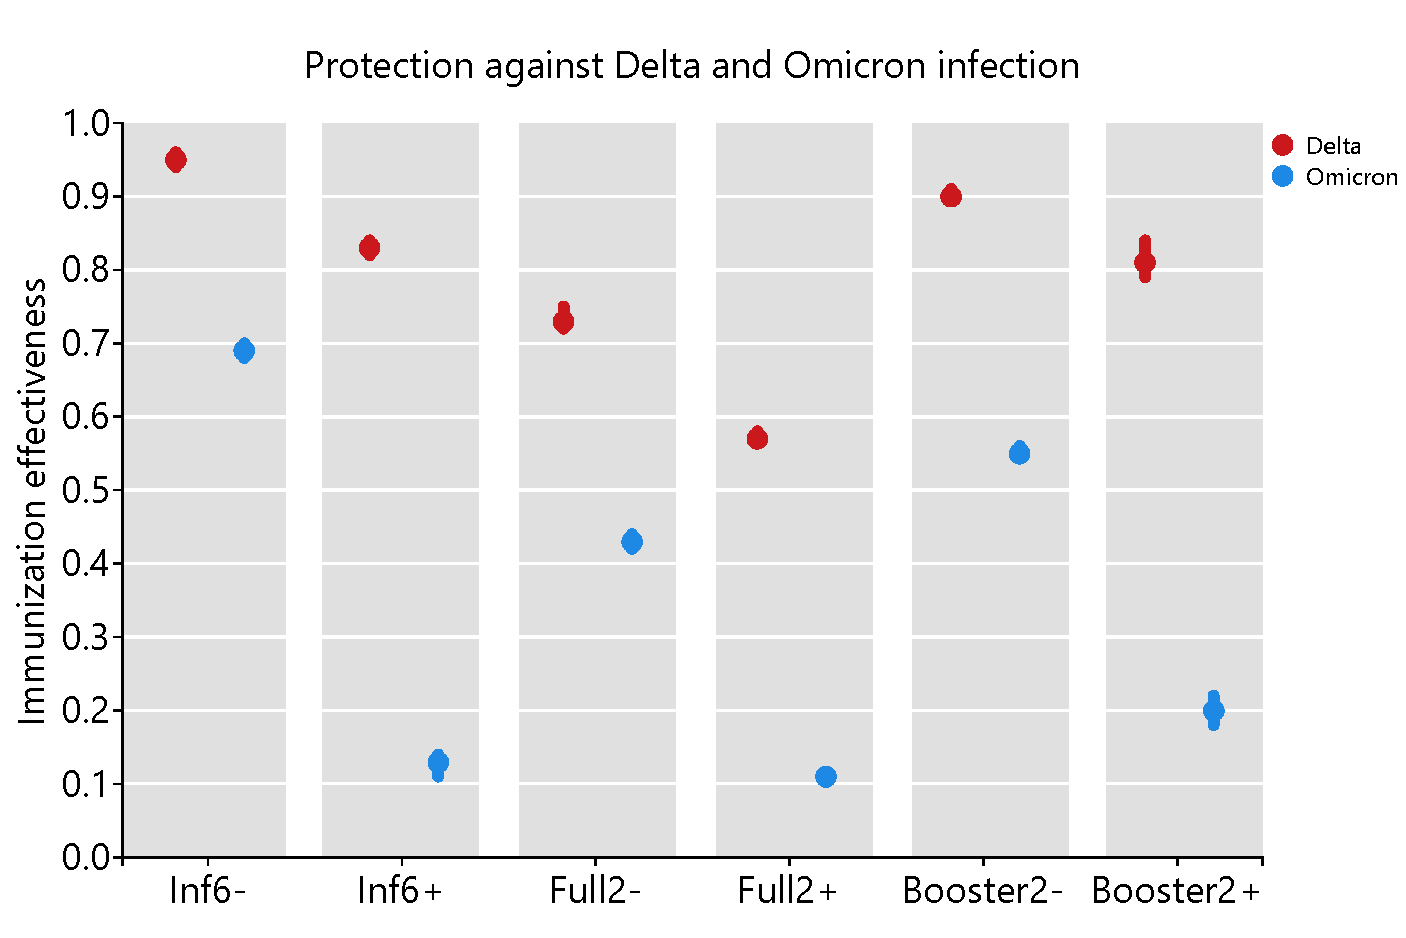
\includegraphics[width=\linewidth]{smid_protection_against_omicron_fig2.pdf}
\caption{Protection provided by vaccination or previous infection against infection by the Omicron and Delta variants of the SARS-CoV-2 virus. Inf6-, previous infection $\leq 6$ months ago; Inf6+, previous infection $>6$ months ago; Full2-, complete vaccination $\leq 2$ months ago;  Full2+, complete vaccination $>2$ months ago; Booster2-, booster dose $\leq 2$ months ago; Booster2+, booster dose $>2$ months ago. Shown are point estimates of protection with 95\% CI.}
\label{figIalone}
\end{figure}
}
We had enough data to examine all the combinations in which a previous infection preceded vaccination. As expected, protection declined with time elapsed from the previous infection or vaccination (Table \tabIinteractions). Regarding protection \new{against} the Delta variant, any combination provided $\geq 95\%$ protection against infection (Table \tabIinteractions). This protection remained quite high also against Omicron when the previous infection was recent, falling to lower values for an older previous infection, but even then the protection was significantly higher than provided by a vaccination or previous infection alone (Table \tabIinteractions). \new{We also analysed cases when a vaccination preceded a previous infection. Regarding Delta for which the protection is generally high, the corresponding value is 96\% (90-98\%) and the order of events thus does not matter. However, for Omicron for which protection is generally lower, the case when a previous infection followed a vaccination appeared to provide a higher protection than the inverse sequence: protection provided by the Full 2+/Inf 6$-$ combination was 89\% (95\% CI 88-91) as compared to 86\% (95\% CI 85-88) for the Inf 6$-$/Full 2+ one.}

\inputtable{smid_protection_against_omicron_tab1.inc}

% These levels of protection against infection provided by vaccination or previous infection were estimated from the complete set of data. 
A finer grained analysis of temporal dynamics of immunity waning after a previous infection was then conducted specifically for individuals that were previously infected but remained non-vaccinated. \new{Against} Omicron, the protection was estimated as 69\% (95\% CI 68-69) for 2-6 months after previous infection,  48\% (95\% CI 46-50) for 7-10 months, 34\% (95\% CI 33-35) for 11-14 months, and 17\% (95\% CI 15-18) for 14 and more months after previous infection. For Delta, on the contrary, these numbers were 93\% (95\% CI 91-94), 91\% (95\% CI 90-92), 86\% (95\% CI 85-86), and 79\% (95\% CI 77-81), respectively.

\subsection*{Protection against hospitalization}

Qualitatively similar pattern yet quantitatively consistently higher protection is seen against hospitalization (Tables \tabHalone), a need for oxygen therapy (Tables \tabOalone), and a need for intensive care (Tables \tabUalone). 
For example, a recent booster dose provides 86\% protection against hospitalization, 90\% against a need of oxygen therapy, and 83\% against a need of intensive care \new{when infected by} the Omicron variant. Moreover, all combinations of previous infection and vaccination present in our data appear to provide nearly complete protection against Omicron as regards hospitalization (Table \tabHinteractions) as well as against need of oxygen therapy or intensive care (often no cases have been observed for such situations, see Supplementary material 2, Sec. 7--10).

\inputtable{smid_protection_against_omicron_tab2.inc}

\inputtable{smid_protection_against_omicron_tab3.inc}

\inputtable{smid_protection_against_omicron_tab4.inc}

% \begin{table}[!ht]
% \caption{Protection due to various combinations of past infection preceding vaccination against hospitalization with a {\it need for oxygen therapy} for the {\it Omicron} variant of the SARS-CoV-2 virus, 95\% confidence intervals (CI) in parentheses. The inverse immunisation order: more than 2 months old vaccination followed by infection in recent 6 months had protection 100\%  (100-100\%)  for booster, and 100\%  (100-100\%) for full vaccination.}
% \label{tabOOinteractions}
% \centering
% \begin{tabular}{|C{.1\linewidth}|C{.16\linewidth}|C{.16\linewidth}|C{.16\linewidth}|C{.16\linewidth}|}
% \hline
% \cellcolor{gray!20}$o \; O_2$&\cellcolor{gray!20}Booster 2-&\cellcolor{gray!20}Full 2-&\cellcolor{gray!20}Booster 2+&\cellcolor{gray!20}Full 2+\\
% \hline
% \cellcolor{gray!20}Inf 6-& $-$ & $-$ & $-$ & $-$ \\
% \hline
% \cellcolor{gray!20}&98\%&100\%&94\%&86\%\\
% \multirow{-2}{*}{\cellcolor{gray!20}Inf 6+}&(93-99\%)&(100-100\%)&(76-98\%)&(75-92\%)\\
% \hline
% \end{tabular} \\[0.5ex]
% \end{table}

% \begin{table}[!ht]
% \caption{Protection due to various combinations of past infection preceding vaccination against hospitalization with a {\it need for oxygen therapy} for the {\it Delta} variant of the SARS-CoV-2 virus, 95\% confidence intervals (CI) in parentheses. The inverse immunisation order: more than 2 months old vaccination followed by infection in recent 6 months had protection 100\%  (100-100\%)  for booster, and 100\%  (100-100\%) for full vaccination.}
% \label{tabODinteractions}
% \centering
% \begin{tabular}{|C{.1\linewidth}|C{.16\linewidth}|C{.16\linewidth}|C{.16\linewidth}|C{.16\linewidth}|}
% \hline
% \cellcolor{gray!20}$\delta \; O_2$&\cellcolor{gray!20}Booster 2-&\cellcolor{gray!20}Full 2-&\cellcolor{gray!20}Booster 2+&\cellcolor{gray!20}Full 2+\\
% \hline
% \cellcolor{gray!20}Inf 6-& $-$ & $-$ & $-$ & $-$ \\
% \hline
% \cellcolor{gray!20}&99\%&97\%&100\%&99\%\\
% \multirow{-2}{*}{\cellcolor{gray!20}Inf 6+}&(98-100\%)&(90-99\%)&(100-100\%)&(98-99\%)\\
% \hline
% \end{tabular} \\[0.5ex]
% \end{table}

\inputtable{smid_protection_against_omicron_tab5.inc}


% \begin{table}[!ht]
% \caption{Protection due to various combinations of past infection preceding vaccination against hospitalization with a need for {\it intensive care} for the {\it Omicron} variant of the SARS-CoV-2 virus, 95\% confidence intervals (CI) in parentheses. The inverse immunisation order: more than 2 months old vaccination followed by infection in recent 6 months had protection 100\%  (100-100\%)  for booster, and 100\%  (100-100\%) for full vaccination.}
% \label{tabUOinteractions}
% \centering
% \begin{tabular}{|C{.1\linewidth}|C{.16\linewidth}|C{.16\linewidth}|C{.16\linewidth}|C{.16\linewidth}|}
% \hline
% \cellcolor{gray!20}$o$ {\it ICU}&\cellcolor{gray!20}Booster 2-&\cellcolor{gray!20}Full 2-&\cellcolor{gray!20}Booster 2+&\cellcolor{gray!20}Full 2+\\
% \hline
% \cellcolor{gray!20}Inf 6-& $-$ & $-$ & $-$ & $-$ \\
% \hline
% \cellcolor{gray!20}&100\%&100\%&100\%&100\%\\
% \multirow{-2}{*}{\cellcolor{gray!20}Inf 6+}&(100-100\%)&(100-100\%)&(100-100\%)&(100-100\%)\\
% \hline
% \end{tabular} \\[0.5ex]
% \end{table}

% \begin{table}[!ht]
% \caption{Protection due to various combinations of past infection preceding vaccination against hospitalization with a need for {\it intensive care} for the {\it Delta} variant of the SARS-CoV-2 virus, 95\% confidence intervals (CI) in parentheses. The inverse immunisation order: more than 2 months old vaccination followed by infection in recent 6 months had protection 100\%  (100-100\%)  for booster, and 100\%  (100-100\%) for full vaccination.}
% \label{tabUDinteractions}
% \centering
% \begin{tabular}{|C{.1\linewidth}|C{.16\linewidth}|C{.16\linewidth}|C{.16\linewidth}|C{.16\linewidth}|}
% \hline
% \cellcolor{gray!20}$\delta$ {\it ICU}&\cellcolor{gray!20}Booster 2-&\cellcolor{gray!20}Full 2-&\cellcolor{gray!20}Booster 2+&\cellcolor{gray!20}Full 2+\\
% \hline
% \cellcolor{gray!20}Inf 6-& $-$ & $-$ & $-$ & $-$ \\
% \hline
% \cellcolor{gray!20}& 100\% & 100\%  & 100\%  & 100\%\\
% \multirow{-2}{*}{\cellcolor{gray!20}Inf 6+}&(100-100\%)&(100-100\%)&(100-100\%)&(97-100\%)\\
% \hline
% \end{tabular} \\[0.5ex]
% \end{table}

\subsection*{Risk of a severe outcome for Omicron vs. Delta}

Finally, our logistic regression analyses show that once infected, the odds ratio for hospitalization with Omicron relative to Delta is 0.36 (0.34-0.38), for a need of oxygen therapy with Omicron relative to Delta is 0.24 (0.22-0.26), and for a need of intensive care with Omicron relative to Delta is also 0.24 (0.21-0.28). Moreover, once hospitalized, the odds ratio for a need of oxygen therapy with Omicron relative to Delta is 0.44 (0.39-0.49) and for a need of intensive care with Omicron relative to Delta is 0.64 (0.52-0.72) (see Supplementary material 2, Sec. 15--19 for further details).

\section*{DISCUSSION}
\label{sec4}

Our data support the existing evidence that the Omicron variant of SARS-CoV-2 evades to a significant extent both the post-vaccination and post-infection immunity \citep{mccallum2022,Dejnirattisai2022,Hoffmann2022,Cui2022,Cao2021}. The VEs of all the vaccines used in the Czech Republic are lower for Omicron compared to Delta. As we previously observed with Alpha and Delta \citep{Berec2021preprint}, the protection against infection by the Omicron variant wanes over time too. However, a booster vaccine dose provides robust and lasting or slowly waning protection against hospitalization, the need for oxygen therapy and intensive care. The combined post-infection and post-vaccination immunity is the most protective regardless of the exact sequence of events, suggesting that the best protective strategy before a coming wave is to vaccinate all individuals, whether previously vaccinated or with a previous covid-19 infection.

We are aware of the complicated interpretation of the hospitalization data for the Omicron wave, as the very high basic reproduction number $R_0$ of this variant \cite{nishiura2022relative} translated into the very high prevalence of infection in the population at the peak of the epidemic wave and a much higher proportion of hospitalized patients with covid-19 as a concomitant finding rather than the reason for admission. We therefore analysed separately the need for oxygen therapy and ICU admission as a more relevant measure of severe outcomes due to the Omicron infection.

Compared to the Delta variant, the protection provided by the post-infection or post-vaccination immunity is lower \new{against} the Omicron variant but at the same time the Omicron variant appears less severe than the Delta variant and the odds ratio for oxygen therapy or ICU admission are both approximately about one quarter compared to the Delta variant.

A common limitation of studies like ours is the fact that only a certain portion of infections is reported (ascertainment rate).  We believe this phenomenon does not affect significantly our estimates of vaccine effectiveness, assuming that the ascertainment rate is the same for the vaccinated and the unvaccinated alike and we have no evidence to the contrary. A potentially low ascertainment rate could also distort our estimates of the protection by the post-infection immunity; in particular, if there were many undetected individuals with post-infection immunity in the control group, the infection risk of the virgin population would be underestimated and, consequently, the protection by infection underestimated as well. Our results should be interpreted in terms of reported infections only. 

\new{We used age and sex as control variables in all our analyses; however, with some caution, they can be as risk factors, too. First of all, the results generally confirm  common knowledge that the risk of various several outcomes grows exponentially with the age -- this is clearly illustrated by the linear increase of log-hazard ratios for both the variants (see Supplementary material 2, Sec. 5--19). The age-related risk of (re-)infection, on the other hand, appears to be for children and the productive age categories. This patter is more stressed for the Omicron variant; however, it is not clear to what extent the pattern is caused by behavioral causes and/or current epidemic situation.}


\subsection*{Notes}

{\bf Data sharing.} 
Data reported in this study and used for the analyses are not public. De-identified individual-level data are available to the scientific community. Requests should be submitted to the Institute of Health Information and Statistics of the Czech Republic  ({\tt www.uzis.cz/index-en.php}), together with a short description of their analysis proposals, where they will be assessed based on relevance and scientific merit.

%{\bf Acknowledgments} We acknowledge ...

%{\bf Contributors} LB, M\v{S}, and LP conceived this study. JJ, OM, JW, MZ, and TB prepared and checked the data, TP provided the methodological expertise, JW and M\v{S} conducted the analyses. LB and JT wrote the first draft of the manuscript. All authors contributed to writing the manuscript and interpreting the results. All authors approved the final version and had final responsibility for the decision to submit for publication. 

{\bf Funding} {\rm No external funding was used to conduct this study.} 

{\bf Potential conflicts of interest} All authors: No reported conflicts. 

%{\bf Data sharing} Data reported in this study and used for the analyses are not public. De-identified individual-level data are available to the scientific community. Requests should be submitted to the Institute of Health Information and Statistics of the Czech Republic \\ ({\tt www.uzis.cz/index-en.php}), together with a short description of their analysis proposals, where they will be assessed based on relevance and scientific merit.

{\bf Corresponding author} {\rm Martin Šmíd, Czech Academy of Sciences, Institute of Information Theory and Automation, Pod Vodárenskou věží 4, 18200 Praha 8, Czech Republic. Mail: smid@utia.cas.cz 


\bibliographystyle{vancouver}
\bibliography{smid_protection_against_omicron_refs}



\end{document}
